\section{Methodology: Spectrum-Matched Circuit Design (SMCD)}
\label{sec:methodology}

\subsection{Setup}

The hybrid ansatz used throughout (the \emph{serial} form; Section~\ref{sec:results}
compares it with a random-scaling variant) is
\[
  x \;\xrightarrow{\;E_\varphi\;}\; z \in \mathbb{R}^m
  \;\xrightarrow{\;Q_\theta\;}\; \phi(z) \in \mathbb{R}
  \;\xrightarrow{\;w\;}\; u(x),
\]
where $E_\varphi$ is an affine classical encoder, $Q_\theta$ a data-re-uploading
variational quantum circuit, and $w$ a linear head. The split is deliberate and is itself
a claim: the classical part learns the coordinate \emph{warping}, the quantum part
supplies the Fourier \emph{basis}, and the head learns the \emph{coefficients} --- exactly
the structure of a spectral method with a learned coordinate map.

\subsection{Proposition 1 --- Circuit spectrum}
\label{sec:prop1}

\begin{proposition}[Circuit spectrum]
An $L$-layer data-re-uploading circuit, with encoding gate $\exp(-ix\,H^{(l)})$ at layer
$l$ for Hermitian generator $H^{(l)}=\sum_a \lambda_a^{(l)}\lvert a\rangle\langle a\rvert$,
realizes an observable expectation of the form
\[
  f(x) \;=\; \sum_{\omega \in \Omega} c_\omega(\theta)\, e^{i\omega x}, \qquad
  \Omega = \left\{ \sum_{l=1}^{L} \left(\lambda^{(l)}_{a_l} - \lambda^{(l)}_{b_l}\right) \right\},
\]
i.e.\ a trigonometric polynomial whose frequency support is the set of all signed
differences of encoding-generator eigenvalues, summed over layers.
\end{proposition}

\paragraph{Proof sketch.} Expand $f(x) = \langle 0\rvert U^\dagger(x,\theta)\, M\,
U(x,\theta)\lvert 0\rangle$ by inserting the eigenbasis resolution of each diagonal
encoding gate independently on the bra and ket sides. Every (bra-path, ket-path) pair
contributes an $x$-dependent phase $\exp\!\big(ix\sum_l(\lambda^{(l)}_{a_l} -
\lambda^{(l)}_{b_l})\big)$ multiplied by an $x$-independent amplitude collecting the
trainable gates and $M$ along that path; collecting paths by total frequency gives the
boxed form. The full derivation, worked first for one qubit/one layer and then generalized
to $n$ qubits and $d$-dimensional inputs, is in \texttt{docs/derivations/07\_circuit\_fourier\_spectrum.md}. $\blacksquare$

\paragraph{Two subtleties that change the constructive guarantee.} Two facts, easy to get
wrong and verified numerically against both an independent statevector simulator and a
PennyLane oracle (agreement $<10^{-10}$) before being trusted:

\begin{enumerate}
\item \textbf{Generator-vs-frequency factor of two.} The generator's eigenvalues are
  $\pm\omega/2$ for an $RZ(\omega x)$ gate, but the \emph{realized} frequency in $f(x)$ is
  the full $\omega$, not $\omega/2$: the eigenvalue-difference structure above supplies a
  compensating factor of two. Reading the generator's eigenvalues off the gate and
  reporting that as the frequency halves every number in the design.
\item \textbf{State-preparation degeneracy.} If the qubit is prepared exactly at the
  equator ($RY(\pi/2)$ before the first encoding gate, an equal superposition), every
  frequency whose balanced-ternary leading digit is zero --- exactly one third of $\Omega$
  --- has identically zero amplitude for \emph{every} trainable-parameter setting,
  independent of ansatz expressivity. This is not a numerical inconvenience: it makes
  Proposition~3 below false for any target spectrum touching a dead frequency under the
  literal $\pi/2$ prescription. We use $\phi_{\mathrm{prep}}=\pi/3$ throughout, verified to
  have no dead frequencies.
\end{enumerate}

\subsubsection{Corollary: ternary scaling and the depth rule}

Set the per-layer scalings to $\omega_l = \Delta\cdot 3^{l-1}$ (single-wire case). Then
$\Omega = \Delta\cdot\{-\tfrac{3^L-1}{2},\dots,\tfrac{3^L-1}{2}\}$ --- exactly $3^L$
distinct frequencies with no degeneracy, a bijection with the balanced-ternary
representation of the integers in that range (proof: substitute $m_l=d_l-1$ to convert the
signed sum into an ordinary base-3 expansion shifted by $\tfrac{3^L-1}{2}$). This grows
\emph{exponentially} in depth, versus $2L+1$ distinct frequencies for linear scaling
$\omega_l=\omega_0$ --- the design knob almost every prior re-uploading paper leaves fixed.

To guarantee the reachable band covers a target maximum frequency $K$ at ternary spacing
$\Delta$:
\[
  \max|\Omega| \ge K
  \iff \Delta\,\tfrac{3^L-1}{2}\ge K
  \iff L \ge \log_3\!\left(\frac{2K}{\Delta}+1\right)
  \;\Longrightarrow\;
  \boxed{L = \left\lceil \log_3\!\left(\tfrac{2K}{\Delta}+1\right)\right\rceil.}
\]
Both the factor of two inside the logarithm and the $+1$ matter. For the Poisson target
spectrum ($K=15\pi$, $\Delta=\pi$), the naive $L=\lceil\log_3(K/\Delta)\rceil$ gives
$L=3$, whose reachable band tops out at $13\pi < 15\pi$ and silently misses the target
mode; the rule above gives $L=4$, whose band reaches $40\pi \ge 15\pi$.

\subsection{Proposition 2 --- PDE target spectrum}

\begin{proposition}[PDE target spectrum]
For a linear constant-coefficient operator $\mathcal{L}$ with Fourier symbol $\sigma(k)$,
the solution of $\mathcal{L}u=f$ on a periodic/rectangular domain satisfies
$\hat u(k) = \hat f(k)/\sigma(k)$. The essential spectral support
$S_\varepsilon = \{k : |\hat u(k)| > \varepsilon\|\hat u\|\}$ is therefore computable
\emph{before training}, from $\hat f$ and $\sigma$ alone.
\end{proposition}

For Helmholtz, $\sigma(k) = k^2 - |\mathbf{k}|^2$, so $S_\varepsilon$ concentrates near
$|\mathbf{k}|\approx k$ --- the near-resonant band a classical PINN's low-frequency-first
learning dynamics reach last, if at all. For the heat equation, $\sigma$ grows
quadratically with $|\mathbf{k}|$ and the solution decays exponentially in time at every
nonzero mode, so $S_\varepsilon$ collapses toward $k=0$ as $t$ increases: this is the
project's negative control (Section~\ref{sec:mechanism}) --- there is little high-frequency
content for a quantum layer to supply, and SMCD predicts this \emph{a priori}, not just
observes it after the fact.

\subsection{Proposition 3 --- Matching condition and resource bound}

\begin{proposition}[Matching \& resource bound]
If $S_\varepsilon \subseteq \Omega$, the hybrid model represents the solution to
$\varepsilon$ accuracy with a linear head --- the remaining optimization problem is convex
in $w$. Covering $S_\varepsilon$ with maximum frequency $K$ and resolution $\Delta$
requires $L \ge \log_3(2K/\Delta+1)$ layers (ternary scaling, above) and
$n \ge \lceil d\rceil$ qubits for $d$ input dimensions, plus ancilla wires for any required
cross-frequency terms.
\end{proposition}

This turns architecture choice into arithmetic: given $(K,\Delta,d)$ read off the PDE's own
symbol and data, $(L,n)$ follow by formula, not by search.

\subsection{Proposition 4 --- NTK consequence}
\label{sec:prop4}

\begin{proposition}[Hybrid NTK decomposition]
For a hybrid model whose parameters $\theta=(\theta_{\mathrm{cl}},\theta_q)$ partition into
disjoint classical and quantum groups,
\[
  \boxed{\Theta_{\mathrm{hyb}}(x,x') \;=\; \Theta_{\mathrm{cl}}(x,x') \;+\; \Theta_q(x,x'),}
\]
exactly, with \textbf{no cross term}; a term of the form $2\Theta_\times$ does not arise
for a shared-output, disjoint-parameter model.
\end{proposition}

\paragraph{Proof.} $\Theta(x,x') = \sum_{k=1}^{P}
\partial_{\theta_k}f(x)\,\partial_{\theta_k}f(x')$ is a single inner product of gradient
\emph{vectors}, summed over the \emph{full} index set of parameters $k=1,\dots,P$. When
that index set is partitioned into two disjoint blocks $\theta_{\mathrm{cl}}$ and
$\theta_q$ (a hybrid model's classical and quantum parameters never overlap), the sum
splits additively over the partition:
\[
  \Theta_{\mathrm{hyb}}(x,x') = \sum_{k\in\mathrm{cl}} \partial_{\theta_k}f(x)\partial_{\theta_k}f(x')
  + \sum_{k\in q} \partial_{\theta_k}f(x)\partial_{\theta_k}f(x')
  = \Theta_{\mathrm{cl}}(x,x') + \Theta_q(x,x').
\]
There is no third term: a cross term would only arise from a fundamentally different
quantity, such as a covariance between two \emph{separately} defined kernels or the square
of a sum of outputs --- not from the NTK of a single model with disjoint parameter groups,
which this project's ansatz is. The identity is also checked numerically on random
synthetic Jacobians of matched and mismatched sizes; \texttt{src/qapinn/xai/ntk.py}
implements it. $\blacksquare$

Because $\Omega$ (the quantum block's realized frequency set) is discrete and prescribed
by construction, $\Theta_q$ has eigen-directions \emph{at} the encoded frequencies with
eigenvalues bounded below independently of $|n|$ for $n\in\Omega$ --- the exponential/power-law
eigenvalue decay in $|k|$ that drives classical spectral bias (Section~\ref{sec:background}) is
replaced by a flat response over $\Omega$. This is the formal statement of ``the quantum
layer removes spectral bias inside its band,'' and it is what Section~\ref{sec:results}'s NTK
spectrum figures measure directly: decay exponent inside $\Omega$ versus outside it, for
matched classical and hybrid models.

\subsection{Algorithm 1 --- SMCD}
\label{sec:algorithm}

\begin{algorithm}[h]
\caption{Spectrum-Matched Circuit Design (SMCD)}
\begin{algorithmic}[1]
\Require PDE operator $\mathcal{L}$, forcing $f$, boundary data $g$, domain
  $\Omega_x$, tolerance $\varepsilon$, qubit budget $n_{\max}$
\Ensure encoding generators \& scalings $\{\omega\}$, depth $L$, qubits $n$,
  entangler, observable, ansatz form
\State \textbf{Symbol:} $\sigma(k) \gets$ Fourier symbol of $\mathcal{L}$ (linearize about a
  base state if nonlinear; Burgers uses the viscous-scale estimate $k_{\max}\sim 1/\sqrt{\nu}$)
\State \textbf{Target:} $\hat S \gets \{k : |\hat f(k)/\sigma(k)| > \varepsilon\} \cup$
  boundary-lift spectral support (time-dependent: union over $t$, record growth rate)
\State \textbf{Band:} $K \gets \max|k|$ in $\hat S$; $\Delta \gets$ min spacing in $\hat S$;
  $d \gets \dim(x)$
\State \textbf{Depth:} $L \gets \lceil \log_3(2K/\Delta + 1)\rceil$ with ternary scalings
  $\omega_j = \Delta\cdot 3^{j-1}$ (Section~\ref{sec:prop1}; fall back to linear
  scaling if $\hat S$ is a dense low band)
\State \textbf{Width:} $n \gets d + n_{\mathrm{cross}}$, where $n_{\mathrm{cross}}$ covers
  required mixed-frequency terms (e.g.\ 2-D Helmholtz needs $k_x\pm k_y$ $\Rightarrow$
  entangle the two coordinate wires)
\If{$n > n_{\max}$ or $L > L_{\max}$ (barren-plateau depth budget)}
  \State split the band into an octave ensemble (Section~\ref{sec:octave})
\EndIf
\State \textbf{Entangler:} ring-CZ if cross terms are needed, else none (unnecessary
  entanglement costs gradient variance for no benefit on a separable target)
\State \textbf{Observable:} local $\langle Z_0\rangle$ (never a global Pauli string ---
  barren plateaus)
\State \textbf{Ansatz:} hard-constrained BCs, $u = B(x) + D(x)\cdot[w\cdot Q_\theta(E_\varphi(x))]$
\State \textbf{Init:} small-angle $\theta\sim\mathcal{N}(0,\sigma_0^2)$, $\sigma_0=0.1$;
  identity-block init for the encoder
\State \textbf{Report:} emit a design card $(\hat S, \Omega, \mathrm{coverage} =
  |\hat S\cap\Omega|/|\hat S|, L, n, \text{param count}, \text{predicted NTK band})$,
  committed alongside every experiment run
\end{algorithmic}
\end{algorithm}

The design card (final step) is what makes the methodology auditable: every run's
predicted coverage can be set against its measured error (Section~\ref{sec:mechanism}).

\subsection{Octave-split circuit ensembles}
\label{sec:octave}

When a single circuit cannot cover $\hat S$ within the barren-plateau depth budget
($L>L_{\max}$), SMCD falls back to $M$ shallow circuits, each matched to one octave band
$[2^j\Delta, 2^{j+1}\Delta)$ of $\hat S$, summed at the head. This keeps every individual
circuit shallow (trainable) while the ensemble covers a wide band --- multi-resolution
analysis with a quantum basis per resolution level.

\subsection{Circuit copies}
\label{sec:copies}

A single circuit reads all of its Fourier amplitudes out through one expectation value,
so every amplitude is a function of the same few angles: changing one frequency's
amplitude moves the others. The copy model removes that coupling without changing the
frequency set. It evaluates $K$ copies of the SMCD circuit on the same encoded input,
each with its own trainable angles, and mixes them with a linear head,
\[
  u(x) = B(x) + D(x)\Big[\,b + \sum_{j=1}^{K} w_j\, Q_{\theta_j}\big(E_\varphi(x)\big)\Big].
\]
Every copy has the same encoding scalings, so the model's frequency set is still exactly
$\Omega$ and every design-card statement above applies unchanged; only the number of
independent handles on the amplitudes grows. $K=1$ is the plain SMCD circuit. On the
one-dimensional problems each copy is a one-qubit, four-layer circuit, and $K=8$ gives
91 trainable parameters. $K$ and the learning rate were selected on tuning seeds before
any held-out run (Section~\ref{sec:setup}).

\paragraph{Why a linear head decouples the amplitudes.} Write the $j$-th copy's output as
a Fourier series over the shared frequency set. The model's amplitude at each frequency is
then a linear combination over copies:
\[
  Q_{\theta_j}(x)=\sum_{\omega\in\Omega}c_\omega(\theta_j)\,e^{i\omega x}
  \quad\Longrightarrow\quad
  \sum_{j=1}^{K} w_j Q_{\theta_j}(x)=\sum_{\omega\in\Omega}\Big(\sum_{j=1}^{K} w_j\,c_\omega(\theta_j)\Big)e^{i\omega x}.
\] With one copy, every $c_\omega$ is fixed by the same ten angles,
and the head can only rescale all of them together. With $K$ copies the head can weight
copies whose angles favour one frequency against copies that favour another, so the
amplitudes at $\pi$ and $15\pi$ can be tuned separately, which is exactly what the
Poisson residual needs (Section~\ref{sec:copyresult}). The parameter count grows
linearly: each copy has 10 angles, the encoder has 2 parameters and the head $K+1$, so
one copy has $10+2+2=14$ parameters and eight copies $80+2+9=91$.

\subsection{A worked design}
\label{sec:worked}

Table~\ref{tab:design} follows Algorithm~1 through the two problems where the method is
tested at full strength. Both designs are computed from the equation and its data alone,
before any training, by \texttt{qapinn.smcd.smcd}.

\paragraph{Poisson.} The forcing of $-u''=f$ with solution $\sin\pi x+0.3\sin15\pi x$ has
two modes, so Proposition~2 gives a target spectrum of exactly two frequencies, $\pi$ and
$15\pi$, with weights 1 and 0.3. The band is $K=15\pi$ and the spacing $\Delta=\pi$, so the
depth rule gives $L=\lceil\log_3(2\cdot15+1)\rceil=\lceil\log_3 31\rceil=4$, since
$3^3=27<31\le81=3^4$. The ternary scalings are $\pi\cdot\{1,3,9,27\}$, and the signed sums
$\pm1\pm3\pm9\pm27$ produce every integer from $-40$ to $40$: 81 frequencies, all multiples
of $\pi$ up to $40\pi$, covering both targets. One input dimension and no cross terms mean
one qubit and no entangler.

\paragraph{Groundwater.} Here the solution is a broad mound from recharge plus six small
ripples from the canals. Its sine series, thresholded at $\varepsilon=10^{-3}$ of the
largest mode, keeps the 32 multiples of $\pi$ from $\pi$ to $32\pi$: the $\pi$ mode carries
most of the weight (the mound), and the canals spread the rest up to $32\pi\approx100$.
Now $K=32\pi$ and $\Delta=\pi$, so $L=\lceil\log_3 65\rceil=4$ again, since $65\le81$. The
same four ternary layers reach $40\pi$ and cover all 32 targets. The two problems need the
same circuit for different reasons: Poisson because of one fast mode at $15\pi$,
groundwater because of many canal harmonics below $32\pi$.

\begin{table}[htbp]
  \centering
  \small
  \begin{tabular}{lll}
  \toprule
  Design step & Poisson & Groundwater \\
  \midrule
  Target spectrum $\hat S$ & $\{\pi, 15\pi\}$ & $\{\pi, 2\pi, \dots, 32\pi\}$ \\
  Band $K$, spacing $\Delta$ & $15\pi$, $\pi$ & $32\pi$, $\pi$ \\
  Depth $L=\lceil\log_3(2K/\Delta+1)\rceil$ & $\lceil\log_3 31\rceil=4$ & $\lceil\log_3 65\rceil=4$ \\
  Scalings & $\pi\cdot\{1,3,9,27\}$ & $\pi\cdot\{1,3,9,27\}$ \\
  Frequency set $\Omega$ & $\pi\cdot\{-40,\dots,40\}$, 81 & $\pi\cdot\{-40,\dots,40\}$, 81 \\
  Coverage $|\hat S\cap\Omega|/|\hat S|$ & 1.0 & 1.0 \\
  Qubits, entangler & 1, none & 1, none \\
  Parameters, 1 copy / 8 copies & 14 / 91 & 14 / 91 \\
  \bottomrule
  \end{tabular}
  \caption{SMCD's design for the two main problems, step by step (Algorithm~1).}
  \label{tab:design}
\end{table}

\begin{figure}[htbp]
\centering
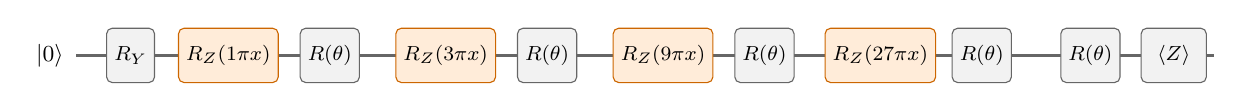
\begin{tikzpicture}[x=1cm, y=1cm, scale=0.92, transform shape,
    gate/.style={draw=black!60, fill=black!5, rounded corners=2pt, minimum height=0.75cm, font=\footnotesize, inner sep=3pt},
    enc/.style={gate, draw=orange!80!black, fill=orange!15}]
  \draw[black!60, thick] (-0.3,0) -- (15.4,0);
  \node[font=\small, anchor=east] at (-0.35,0) {$|0\rangle$};
  \node[gate] at (0.45,0) {$R_Y$};
  \foreach \s/\x in {1/1.8, 3/4.8, 9/7.8, 27/10.8} {
    \node[enc] at (\x,0) {$R_Z(\s\pi x)$};
    \node[gate] at (\x+1.4,0) {$R(\theta)$};
  }
  \node[gate] at (13.7,0) {$R(\theta)$};
  \node[gate, minimum width=0.9cm] at (14.85,0) {$\langle Z\rangle$};
\end{tikzpicture}
\caption{One copy of the SMCD circuit for both problems: state preparation, four
  re-uploading layers whose encoding gates (orange) carry SMCD's scalings, trainable
  rotations (grey), and a local $Z$ measurement.}
\label{fig:circuit}
\end{figure}
